\documentclass[11pt]{article}
\usepackage[margin=1in]{geometry}
\usepackage{amsmath,amssymb,amsthm,booktabs,graphicx,float}
\usepackage[hidelinks]{hyperref}
\usepackage{parskip}

\graphicspath{{../results/}}
\newtheorem{proposition}{Proposition}
\newcommand{\E}{\mathbb{E}}
\newcommand{\1}{\mathbf{1}}
\newcommand{\ctrig}{c_{\mathrm{trig}}}
\newcommand{\bmda}{\bar c_{\mathrm{MDA}}}

\title{Pricing AT1 Contingent Convertibles as a Claim on Bank Capital\\[4pt]
\large Model, numerical method, and a calibration to BNP Paribas's USD AT1s}
\author{Paolo Mastrogiacomo \\ \texttt{Credit-Quant-Research / at1-coco-pricer}}
\date{September 2026}

\begin{document}
\maketitle

\begin{abstract}
An Additional Tier~1 (AT1) bond is a perpetual, deeply subordinated bank bond
whose cash flows depend on the issuer's capital: coupons are cut when capital
enters the regulatory buffer, principal is converted or written down at a
capital trigger or at the regulator's discretion, and the issuer calls only when
refinancing is cheaper. We take the Common Equity Tier~1 (CET1) ratio as the
state variable, add a mean-reverting issuer spread that drives both the call
decision and the regulatory write-down (PONV) hazard, and price by Monte Carlo
with the PONV hazard integrated analytically along each path. Calibrated to
BNP Paribas's three USD AT1s (September 2026), with the FRED Treasury curve
and 50 quarters of CET1 history, one implied hazard of about $2.3\%$ a year
prices all three bonds. About $240$bp of the $\approx 270$--$280$bp spread is
compensation for PONV, tail and liquidity risk; mechanical conversion explains
$\approx4$bp. The price is flat in capital above the MDA threshold
($\approx0.45$ points per point of CET1) and steep around it ($\approx4$
points). A bootstrap shows that the speed of capital mean reversion is the
weakest input: the half-life of a capital shock is anywhere between 1.5 and 11
years, and the capital stress results scale by a factor of six across that
range. The bond cross-section is consistent only with the faster end, which
sets the base case.
\end{abstract}

\tableofcontents

%======================================================================
\section{The instrument and the idea}
%======================================================================

\subsection{What an AT1 is}
An AT1 bond counts as going-concern regulatory capital for a bank. Its terms
make it behave partly like equity:
\begin{enumerate}
  \item \textbf{Perpetual, with issuer calls.} There is no maturity. The issuer
  may redeem at par on call dates; for the bonds studied here, only on
  \emph{reset dates}, every five years from the first call. If not called, the
  coupon resets to a reference rate (5-year US Treasury, CMT) plus the margin
  fixed at issue. Investors are exposed to \emph{extension}: the issuer calls
  when it is cheap to refinance, and does not when it is expensive, which is
  exactly when investors would want their money back.
  \item \textbf{Discretionary, non-cumulative coupons.} Coupons may be cancelled
  at any time and are lost for good. They are also mechanically restricted when
  CET1 falls inside the \emph{combined buffer requirement}: the Maximum
  Distributable Amount (MDA) rule of CRD~IV.
  \item \textbf{Loss absorption.} If CET1 falls below a contractual trigger
  ($5.125\%$ here), the bond converts into shares (or is written down). The
  resolution authority can also impose losses at the \emph{Point of
  Non-Viability} (PONV) while CET1 is still above the trigger: Credit Suisse's
  AT1s were written to zero in March 2023 with a reported CET1 ratio of about $14\%$.
\end{enumerate}

\subsection{Why capital is the state variable}
Trigger, coupon restriction and (partly) the call decision are all written on
the CET1 ratio. Modelling CET1 directly makes these three risks consistent by
construction: the same simulated path that approaches the MDA threshold also
cuts coupons, discourages a call, and raises the chance of loss absorption.
The alternative, an equity-barrier model, needs a mapping from share price to
capital that is unobservable and unstable.

Capital alone is not enough, however. The market prices AT1s far below what
historical capital volatility would justify (\S\ref{sec:results}), and the
call decision depends on market spreads, not only on capital. We therefore add
a second state variable, the issuer's AT1 spread, which (i) drives the call
decision and (ii) scales the PONV hazard.

%======================================================================
\section{State dynamics}
%======================================================================

\subsection{CET1 ratio}
Let $C_t$ be the CET1 ratio in percentage points. We use a mean-reverting
jump-diffusion with downward jumps:
\begin{equation}\label{eq:cet1}
  dC_t = \kappa(\theta - C_t)\,dt + \sigma\,dW_t - J\,dN_t,
\end{equation}
where $N_t$ is a Poisson process with intensity $\lambda_J$ (stress events) and
jump sizes are i.i.d.
\[
  J = m_J \exp\!\bigl(\sigma_J Z - \tfrac12\sigma_J^2\bigr),\qquad Z\sim N(0,1),
  \qquad \E[J]=m_J .
\]
Mean reversion to $\theta$ represents the bank's capital management (retained
earnings, distribution policy, management of risk-weighted assets); the target
$\theta$ is management's stated CET1 objective. Jumps are one-sided because
losses arrive suddenly while recapitalisation is gradual.

The \emph{mechanical trigger time} is
$\tau_m = \inf\{t:\ C_t \le \ctrig\}$.

\subsection{Issuer AT1 spread}
Let $S_t$ be the market level of the issuer's new-issue AT1 spread (decimal).
It follows an Ornstein--Uhlenbeck process correlated with capital shocks,
\begin{equation}\label{eq:spread}
  dS_t = a(\bar s - S_t)\,dt + \eta\,dB_t,\qquad
  d\langle B, W\rangle_t = \rho\,dt,\quad \rho<0,
\end{equation}
and the issuer's \emph{effective} spread adds a capital premium once CET1 is
inside the buffer:
\begin{equation}\label{eq:seff}
  s_t = S_t + \beta\,\bigl(\bmda - C_t\bigr)^+ ,
\end{equation}
where $\bmda$ is the MDA threshold defined below. The effective spread $s_t$ is
the rate at which the bank could issue a new AT1 at time $t$.

%======================================================================
\section{Contract features as functionals of the state}
%======================================================================

\subsection{MDA coupon restriction}
Let $b$ be the MDA floor (Pillar~1 plus the CET1 part of Pillar~2R) and $w$ the
combined buffer (conservation, systemic and countercyclical buffers), so that
$\bmda=b+w$. With $q=(C-b)/w$ the position inside the buffer, the fraction of
the scheduled coupon that can be paid is
\begin{equation}\label{eq:mda}
  \phi(C)=
  \begin{cases}
    1 & C \ge b+w,\\
    0.6 & q\in[0.75,1),\\
    0.4 & q\in[0.50,0.75),\\
    0.2 & q\in[0.25,0.50),\\
    0 & q<0.25 \ \text{or}\ C<b.
  \end{cases}
\end{equation}
This is a stylised version of the quartile schedule; it makes
coupon-cancellation risk emerge from the same paths as trigger risk.

\subsection{Call and extension}
Let $T_1<T_2<\dots$ be the reset (call) dates and $m$ the reset margin over the
5-year reference rate. The issuer calls at the first reset date $T_k$ at which
\begin{equation}\label{eq:call}
  m > s_{T_k}
  \qquad\text{and}\qquad C_{T_k}\ge \bmda
  \qquad\text{and}\qquad T_k<\tau_m ,
\end{equation}
that is, when keeping the bond costs more than issuing a new one, provided the
regulator would approve the call (CET1 above the MDA threshold) and the bond is
still alive. Denote the call time by $\tau_c$ ($+\infty$ if never). If
$\eta>0$ the call is random even for a healthy bank; the low-margin bond is the
first to be extended when spreads widen.

\subsection{Conversion}
At $\tau_m$ the bond converts into shares at the higher of the market price
and a floor price $P_{\mathrm{floor}}$. The investor receives shares worth
$F\cdot S^{\mathrm{eq}}_{\tau_m}/P_{\mathrm{floor}}$ (when the share trades
below the floor, as it will at the trigger). The model uses a stressed share
price $S^{\mathrm{eq}}_{\tau_m} = \xi\, S^{\mathrm{eq}}_0 X_0$ (converted to
USD at $X_0$), so the recovery is
\begin{equation}
  R = \min\!\left(1,\ \frac{\xi\,S^{\mathrm{eq}}_0 X_0}{P_{\mathrm{floor}}}\right).
\end{equation}

\subsection{PONV: a hazard linked to the spread}
The regulator may impose losses before the trigger. We model this as a
doubly-stochastic (Cox) event with intensity proportional to the effective
spread,
\begin{equation}\label{eq:hazard}
  \lambda_t = \lambda\,\frac{s_t}{s_0},
\end{equation}
so $\lambda$ is today's hazard, and the hazard rises when spreads widen or
capital falls inside the buffer. Recovery at PONV is zero. Linking the hazard to
$s_t$ is what makes extension consistent: the states in which the issuer
extends ($s_t>m$) are exactly those in which the bond is riskier and worth less.
With a constant hazard, extension would be valued at a discount rate that does
not reflect the state, and could even look valuable to the investor.

%======================================================================
\section{Valuation}
%======================================================================

\subsection{Pricing equation}
Let $r$ be the flat, continuously compounded risk-free rate, $F$ the face and
$t_i$ the coupon dates, paid at frequency $f$. The scheduled coupon is
$c(t_i)=c_0$ up to and including $T_1$ and $c(t_i)=y^{\mathrm{ref}}+m$ after it.
Let $\tau_P$ be the PONV time. The dirty price is
\begin{equation}\label{eq:price}
\begin{split}
  V_0=\E\Biggl[\,&\sum_{t_i}\1_{\{t_i<\tau_m,\ t_i\le\tau_c,\ t_i<\tau_P\}}
  \frac{\phi(C_{t_i})\,c(t_i)\,F}{f}\,e^{-rt_i}
  + \1_{\{\tau_c<\tau_m,\ \tau_c<\tau_P\}}\,F\,e^{-r\tau_c}\\
  &+ \1_{\{\tau_m<\tau_c,\ \tau_m<\tau_P\}}\,R\,F\,e^{-r\tau_m}\Biggr]
  + \text{tail}.
\end{split}
\end{equation}
Paths alive at the horizon $H=40$ years receive the value of a perpetuity at
the reset coupon, $F(y^{\mathrm{ref}}+m)/(r+\lambda_H)$, discounted to today.

\subsection{Conditional Monte Carlo for the PONV hazard}
\begin{proposition}
Let $\mathcal{G}$ be the $\sigma$-algebra generated by the paths of $(C,S)$.
Conditional on $\mathcal G$, the PONV time has intensity \eqref{eq:hazard}, so
\[
  \Pr(\tau_P>t\mid\mathcal G)=\exp\!\Bigl(-\lambda\int_0^t \frac{s_u}{s_0}\,du\Bigr)
  \equiv e^{-\lambda I_t}.
\]
Hence
\begin{equation}\label{eq:cmc}
  V_0(\lambda)=\E\Biggl[\,\sum_{t_i}\mathrm{CF}_i\,e^{-rt_i-\lambda I_{t_i}}
  + \mathrm{CF}_{\mathrm{end}}\,e^{-rT_{\mathrm{end}}-\lambda I_{T_{\mathrm{end}}}}\Biggr],
\end{equation}
where $\mathrm{CF}_i$ are the coupon cash flows and $\mathrm{CF}_{\mathrm{end}}$
is the call, conversion or tail payment at the end of each path's life, all
computed without reference to $\tau_P$.
\end{proposition}
\begin{proof}
Condition each indicator $\1_{\{t<\tau_P\}}$ in \eqref{eq:price} on
$\mathcal G$ (tower property); every other term is $\mathcal G$-measurable.
\end{proof}

Consequences for the numerics:
\begin{itemize}
  \item PONV is never simulated as an event, which removes its sampling noise
  (Rao--Blackwellisation).
  \item On a fixed set of paths, $V_0(\lambda)$ is smooth and strictly decreasing
  in $\lambda$ (because $I_t>0$). The market-implied hazard is therefore the unique root of
  $V_0(\lambda)=P^{\mathrm{clean}}+\mathrm{AI}$ and is found with Brent's method.
  \item Cash flows and $I_t$ are stored per path once; each evaluation of
  $V_0(\lambda)$ is a vectorised sum.
\end{itemize}

\subsection{Discretisation}
The grid is monthly ($\Delta=1/12$) over 40 years, with 20{,}000 paths.
CET1 uses an Euler step with a Bernoulli jump of probability
$1-e^{-\lambda_J\Delta}$; the spread uses the exact OU transition
\[
  S_{n+1}=\bar s+(S_n-\bar s)e^{-a\Delta}
  +\eta\sqrt{\tfrac{1-e^{-2a\Delta}}{2a}}\,
  \bigl(\rho Z^C_n+\sqrt{1-\rho^2}\,Z^\perp_n\bigr).
\]
Coupons are discounted at their exact dates; path events (trigger, call) are
read on the grid. Market prices are clean, so the model value is compared with
the clean price plus 30/360 accrued interest (the accrued amount matches Capital
IQ to three decimals).

\subsection{Common random numbers}
All primitive random numbers are drawn once and reused across scenarios,
bumps and feature switches. Differences between two prices (Greeks, stress
P\&L, spread components) therefore carry no Monte Carlo noise of their own.

%======================================================================
\section{Calibration}\label{sec:calib}
%======================================================================

\subsection{Capital dynamics from history}
The CET1 series is quarterly from 2014Q1 to 2026Q2 (50 observations). Earlier
data follow Basel~II/2.5 definitions and are not comparable. The 2023Q1 change
(+1.2pp, sale of Bank of the West) is a disposal, not a capital shock, and that
transition is excluded from the likelihood. The OU transition density is
Gaussian for any step $\Delta_k$,
\[
  C_{k+1}\mid C_k \sim N\!\Bigl(\theta+(C_k-\theta)e^{-\kappa\Delta_k},\
  \tfrac{\sigma^2}{2\kappa}\bigl(1-e^{-2\kappa\Delta_k}\bigr)\Bigr),
\]
so the likelihood is exact. Fixing $\theta=13\%$ (BNP's target) gives
$\hat\kappa=0.165$ and $\hat\sigma=0.44$pp$/\sqrt{\text{yr}}$; $\kappa$ is weakly
identified and the base case uses $\kappa=0.35$ (\S\ref{sec:uncert}), with
$\sigma=0.47$ re-estimated given $\kappa$. The 2014Q2 fall of $0.76$pp (US
sanctions settlement) is an example of the stress events the jumps represent. The jumps
cannot be identified from this sample; we use $\lambda_J=0.12$, $m_J=2.2$pp,
$\sigma_J=0.5$, whose 95th-percentile jump (4.4pp) matches BNP's CET1 depletion
in the EBA 2025 adverse scenario (4.2pp, fully loaded).

\subsection{Regulatory geometry}
From the 2025 requirement stack, $b=4.5+1.14=5.64\%$ and
$w=2.5+1.5+0.73+0.14=4.87\%$ (conservation, G-SIB, countercyclical and
systemic-risk buffers), so $\bmda=10.51\%$. The trigger is $\ctrig=5.125\%$ of
group CET1.

\subsection{Market inputs}
The inputs are:
\begin{itemize}
  \item the clean price of each bond (Capital IQ evaluated prices);
  \item the FRED constant-maturity Treasury curve (DGS5, DGS7, DGS10): the 5-year
  CMT is the reset reference, and each bond is discounted at the yield
  interpolated at its first call date;
  \item the AT1 spread $S_0$, the average of (bond yield $-$ call-matched Treasury);
  \item the latest published CET1 ratio, with a 35-day publication lag;
  \item the share price.
\end{itemize}
The spread process uses $a=0.5$, $\bar s$ equal to the sample mean (275bp),
$\eta=100$bp and $\rho=-0.3$; the capital premium is $\beta=1\%$ per point of CET1 and the share
stress is $\xi=0.2$.

\subsection{Implied hazard and cross-sectional identification}
For each date and bond $j$ we solve $V_0^{(j)}(\lambda_j)=P_j$. The three bonds
share issuer, capital and trigger, so a correct model should give
$\lambda_1=\lambda_2=\lambda_3$. The dispersion
$D=\max_j\lambda_j-\min_j\lambda_j$ is a specification test, and it can be
used to ask which values of the other parameters (the spread volatility $\eta$,
the capital mean reversion $\kappa$) the three prices are consistent with.

%======================================================================
\section{Analytics}
%======================================================================

\subsection{Spread decomposition}
Switch the features on one at a time and convert each price into a yield to the
first call date, $y^{(k)}$ (semi-annual, bullet to $T_1$):
\begin{center}
\begin{tabular}{cl}
\toprule
$k$ & price $V^{(k)}$ \\
\midrule
0 & certain call at $T_1$, full coupons, no conversion, $\lambda=0$ (risk-free) \\
1 & + PONV hazard $\lambda$ \\
2 & + MDA coupon restriction \\
3 & + conversion at the trigger \\
4 & + economic call rule \eqref{eq:call} \ $=$ market price \\
\bottomrule
\end{tabular}
\end{center}
Because $V^{(0)}$ is discounted at $r$, $y^{(0)}$ is the Treasury yield, and the
increments $y^{(k)}-y^{(k-1)}$ telescope to the market yield-to-call spread. The
order is chosen so that every feature is valued with risky discounting and
extension comes last, with all other features in place.

\subsection{Call probability and the cost of the call option}
$\Pr(\tau_c=T_1)$ is read from the paths. The cost of the issuer's option is
$V^{\mathrm{call\ at\ }T_1}-V$. Negative convexity is measured as the extra loss
for a $+50$bp shift in the spread level (with the hazard scaled accordingly),
relative to a bond whose call at $T_1$ is certain.

\subsection{Stress and capital delta}
Each scenario shifts $C_0$, the spread ($S_0$ and $\bar s$, with $\lambda$ scaled
by $S$) or the Treasury level, and reprices on the same paths. The capital delta
$\partial V/\partial C_0$ is a finite difference on a grid of $C_0$.

%======================================================================
\section{Results: BNP Paribas, 25 September 2026}\label{sec:results}
%======================================================================

\subsection{Capital}
\begin{figure}[H]
\centering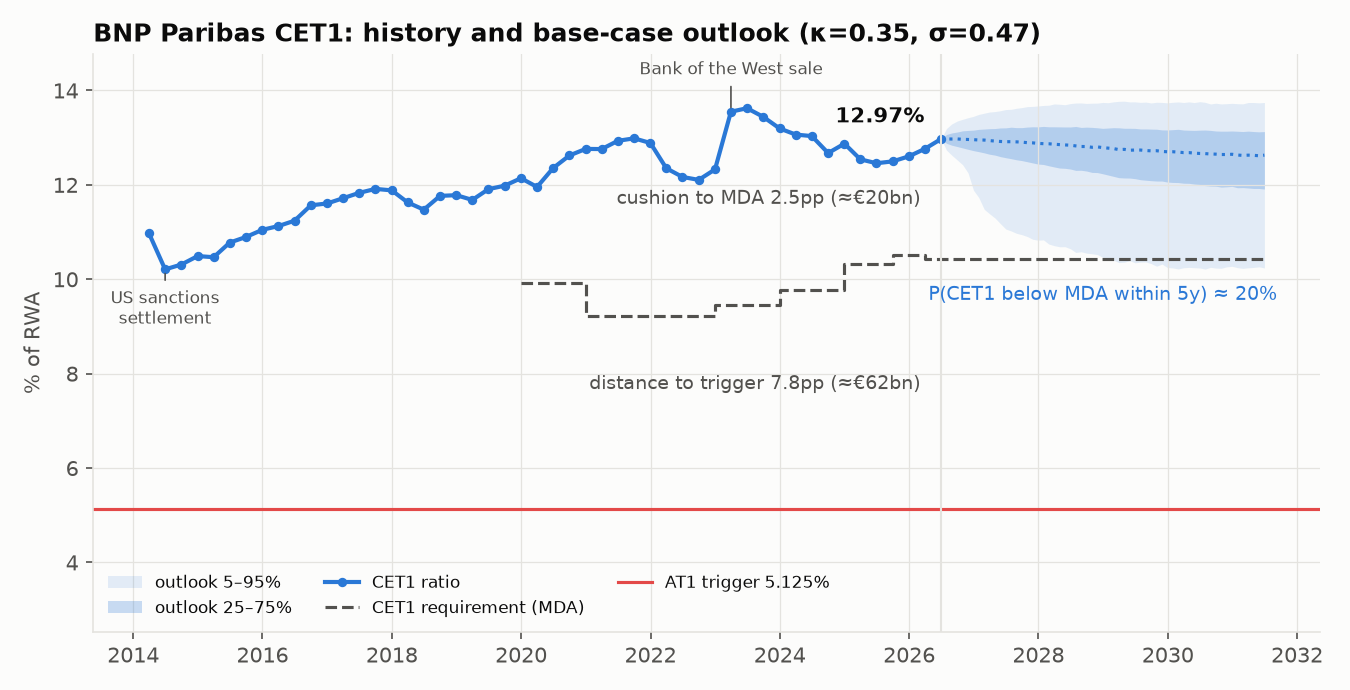
\includegraphics[width=0.8\textwidth]{bnp_cet1_history.png}
\caption{CET1 ratio since 2014, CET1 requirement (MDA threshold), AT1 trigger and
the base-case 5-year outlook (median, 50\% and 90\% bands of the simulated CET1).}
\end{figure}
CET1 was $12.97\%$ at June 2026 against a $10.43\%$ requirement: a cushion of
$2.5$pp ($\approx$\,EUR~20bn). The trigger is $7.8$pp lower
($\approx$\,EUR~62bn of losses). Under the base-case dynamics, about $20\%$ of the
simulated paths fall below the MDA threshold at some point in the next five
years, while the trigger is almost never reached by diffusion alone: capital
risk for these bonds is first a coupon risk, then a conversion risk.

\subsection{The three bonds and the implied hazard}
\begin{table}[H]
\centering
\begin{tabular}{lccc}
\toprule
 & 6.875\% NC33 & 7.20\% NC36 & 7.45\% NC35 \\
\midrule
Reset margin (bp) & 285 & 294 & 313 \\
Clean price & 94.39 & 95.25 & 97.57 \\
Model price with $\lambda=0$ & 114.8 & 117.6 & 118.2 \\
Implied hazard $\lambda$ (\%/yr) & 2.33 & 2.31 & 2.31 \\
$\Pr(\text{called at } T_1)$ & 51\% & 53\% & 60\% \\
Lifetime $\Pr(\text{conversion})$ & 1.3\% & 1.5\% & 1.3\% \\
\bottomrule
\end{tabular}
\caption{Last date, base case ($\kappa=0.35$, $\eta=100$bp).}
\end{table}

Dispersion of the implied hazards across the three bonds, by spread volatility:
\begin{center}
\begin{tabular}{lccccccc}
\toprule
$\eta$ (bp) & 0 & 25 & 50 & 75 & 100 & 150 & 200\\
\midrule
$D(\eta)$ (bp of hazard) & 8.3 & 6.0 & 4.1 & 2.9 & \textbf{2.3} & 1.5 & 1.0\\
\bottomrule
\end{tabular}
\end{center}
A stochastic refinancing spread is clearly needed (8.3bp with a deterministic
one), but the dispersion keeps falling as $\eta$ rises, so the cross-section does
not pin $\eta$ down; $100$bp is kept as an assumption. Over 66 weekly dates the
mean dispersion is $6.0$bp against $9.6$bp for the deterministic rule. With
Capital IQ benchmark proxies instead of the FRED curve the last-date dispersion
is $2.7$--$7.6$bp.

\begin{figure}[H]
\centering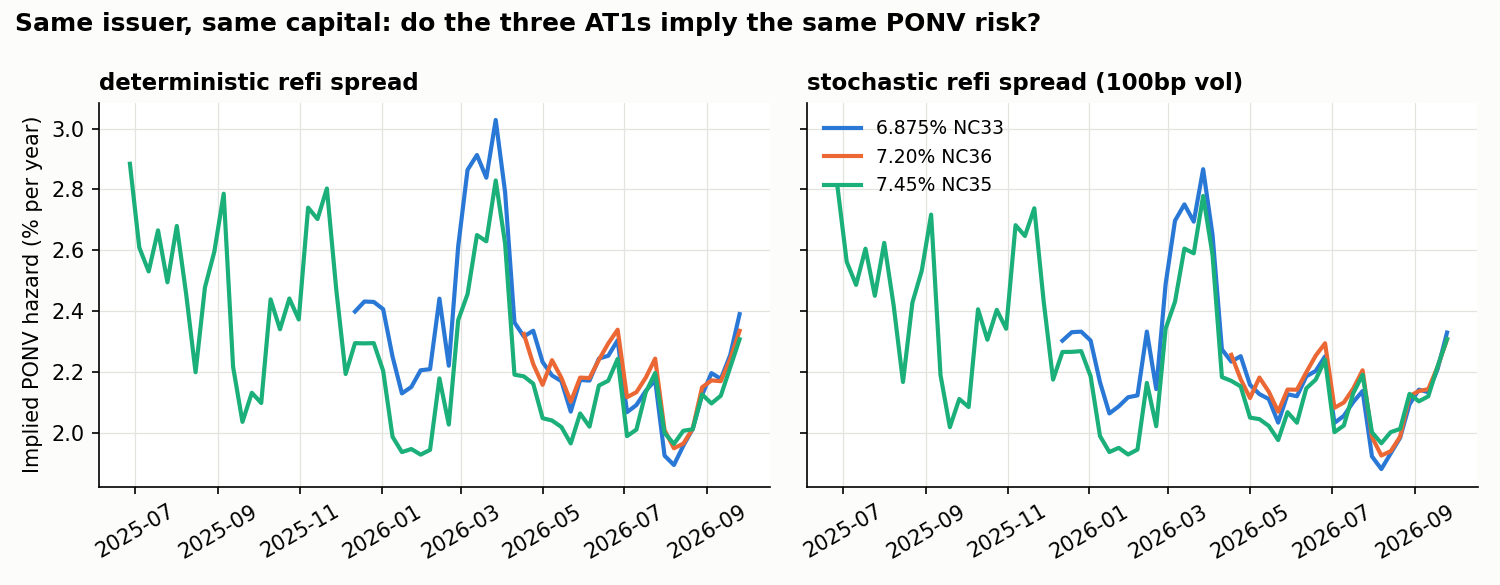
\includegraphics[width=\textwidth]{implied_ponv.png}
\caption{Implied PONV hazard per bond, weekly.}
\end{figure}

\subsection{What the spread pays for}
\begin{table}[H]
\centering
\begin{tabular}{lccc}
\toprule
bp of yield-to-call spread & 6.875\% NC33 & 7.20\% NC36 & 7.45\% NC35 \\
\midrule
PONV / tail / liquidity & 243 & 240 & 239 \\
MDA coupon cuts & 20 & 22 & 22 \\
Conversion at the trigger & 4 & 5 & 4 \\
Extension & 12 & 7 & 4 \\
\midrule
Total $=$ market & 279 & 274 & 269 \\
\bottomrule
\end{tabular}
\end{table}
\begin{figure}[H]
\centering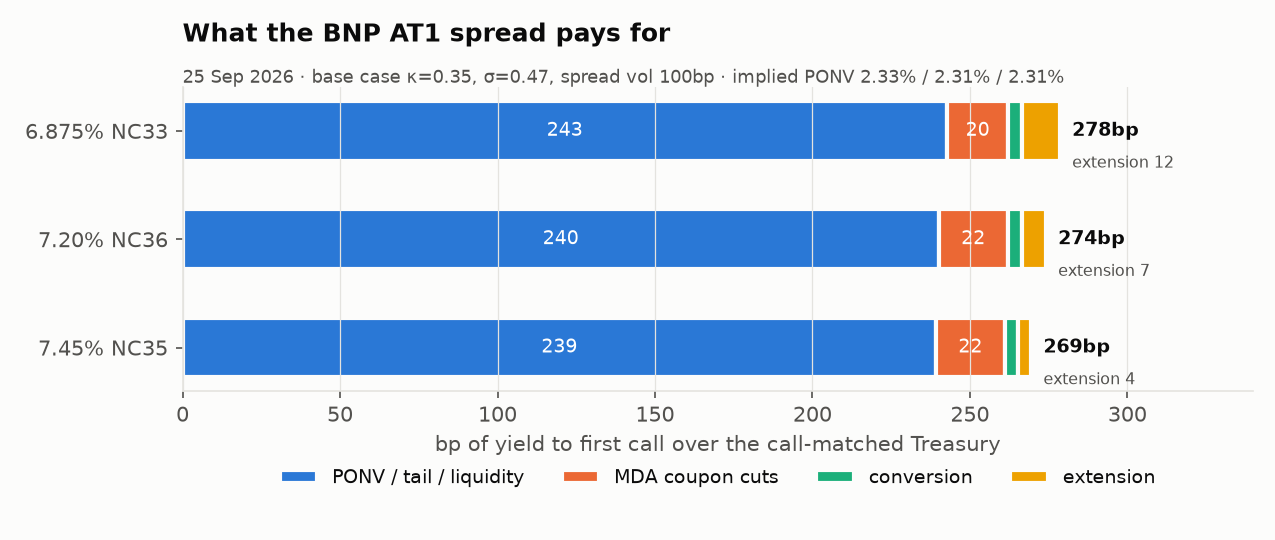
\includegraphics[width=0.85\textwidth]{spread_decomposition.png}
\end{figure}
With BNP's capital dynamics, mechanical conversion is a 1.3--1.5\% lifetime
event worth $\approx4$bp. Almost all of the spread is
compensation for regulatory write-down before the trigger, tail risk beyond the
historical sample, and liquidity. The extension component decreases with the
reset margin, as the theory requires. The split between the premium and the
MDA component depends on $\kappa$ (\S\ref{sec:uncert}); the total does not.

\subsection{Call and extension}
\begin{table}[H]
\centering
\begin{tabular}{lccc}
\toprule
 & 6.875\% NC33 & 7.20\% NC36 & 7.45\% NC35 \\
\midrule
Margin $-$ today's AT1 spread (bp) & $+6$ & $+15$ & $+34$ \\
Cost of the issuer's option (pts) & 0.63 & 0.47 & 0.26 \\
P\&L, spreads $+50$bp (pts) & $-3.4$ & $-3.6$ & $-3.3$ \\
\quad of which from extension (pts) & $-1.2$ & $-0.9$ & $-0.7$ \\
\bottomrule
\end{tabular}
\end{table}
\begin{figure}[H]
\centering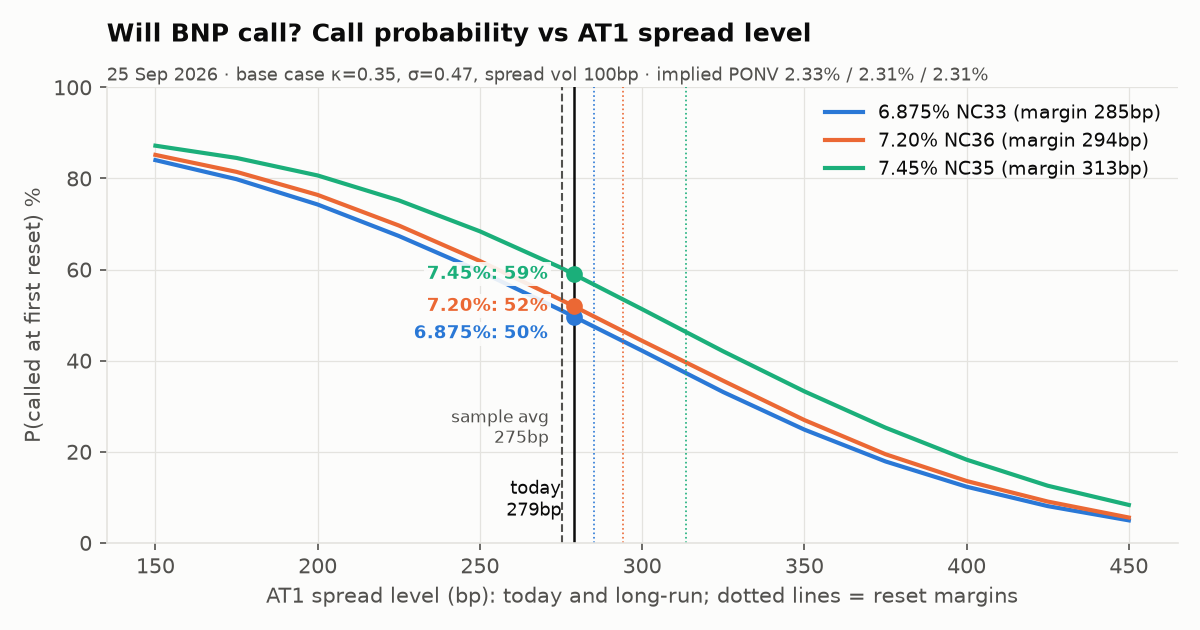
\includegraphics[width=0.8\textwidth]{call_probability.png}
\end{figure}
The low-margin bond is the most negatively convex. In the four weeks to 25 September 2026 the 10y Treasury rose $45$bp; on top of
that, the spread of the 6.875\% widened by $34$bp, against $10$--$12$bp for the
other two.

\subsection{Stress and the capital cliff}
\begin{table}[H]
\centering
\begin{tabular}{lccc}
\toprule
Clean price change (points) & 6.875\% NC33 & 7.20\% NC36 & 7.45\% NC35 \\
\midrule
Rates $+100$bp & $-5.2$ & $-6.3$ & $-6.1$ \\
CET1 $-2$pp & $-1.2$ & $-1.2$ & $-1.2$ \\
CET1 $-4.2$pp (EBA adverse) & $-8.3$ & $-9.5$ & $-8.9$ \\
AT1 spreads $+200$bp & $-16.9$ & $-16.8$ & $-16.0$ \\
EBA adverse $+$ spreads $+200$bp & $-24.6$ & $-25.6$ & $-24.2$ \\
PONV hazard $\times3$ & $-26.8$ & $-29.0$ & $-27.9$ \\
\bottomrule
\end{tabular}
\end{table}
\begin{figure}[H]
\centering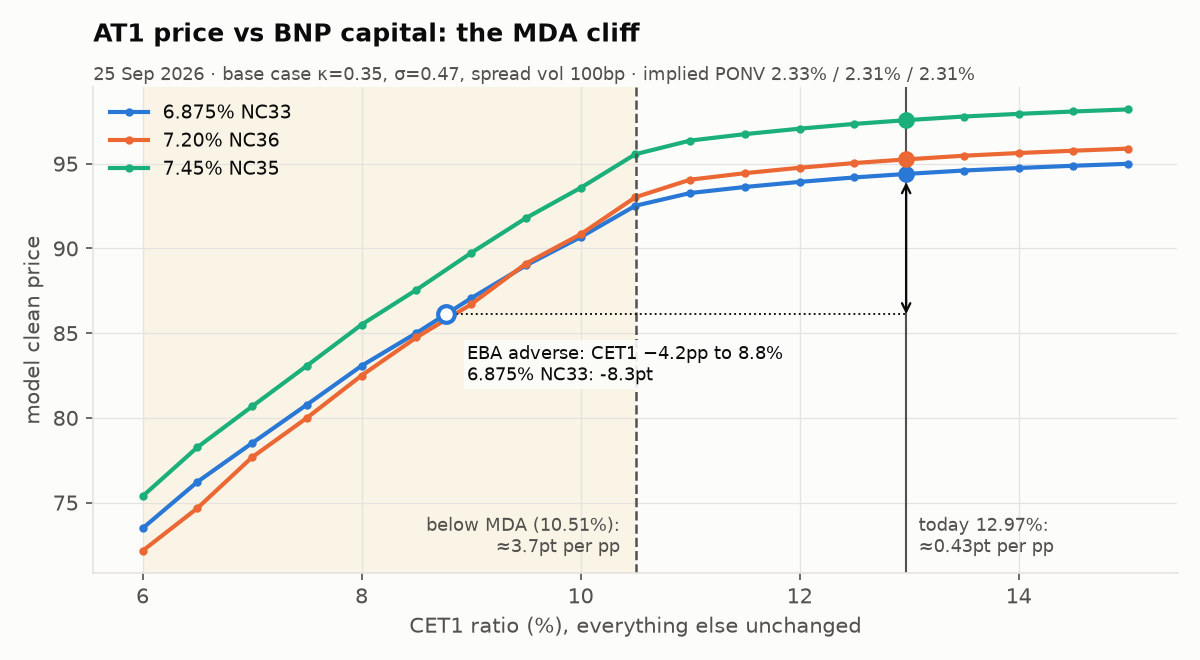
\includegraphics[width=0.8\textwidth]{price_vs_cet1.png}
\end{figure}
The capital delta is $\approx0.45$ points per point of CET1 at $13\%$ and
$\approx4$ around and below the MDA threshold. Crossing $\bmda$ switches on three
mechanisms at once: coupons are cut by \eqref{eq:mda}, the call is blocked by
\eqref{eq:call}, and the hazard rises through \eqref{eq:seff}--\eqref{eq:hazard}.
For risk management, the distance that matters is the distance to the MDA
threshold, not to the trigger.

\subsection{How much can we trust the capital parameters?}\label{sec:uncert}
\textbf{Bootstrap.} We simulate 1{,}000 CET1 histories on the observed quarterly
dates with the fitted dynamics and re-estimate $(\kappa,\sigma)$ on each. The 90\%
intervals are $\kappa\in[0.06,\,0.48]$ and $\sigma\in[0.37,\,0.52]$: volatility
is well estimated, the speed of capital rebuilding is not. The half-life of a
capital shock, $\ln 2/\kappa$, lies between 1.5 and 11 years (point estimate 4.2).

\begin{table}[H]
\centering
\begin{tabular}{lcccc}
\toprule
Average of the three bonds & $\kappa=0.06$ & $\kappa=0.165$ & $\kappa=0.35$ & $\kappa=0.48$ \\
 & (5\%) & (history) & (base) & (95\%) \\
\midrule
Implied PONV (\%/yr) & 0.9 & 1.9 & 2.3 & 2.4 \\
MDA coupon cost (pts) & 10.9 & 4.4 & 1.7 & 1.2 \\
Capital delta at the MDA threshold (pts/pp) & 12.9 & 7.0 & 3.3 & 2.3 \\
EBA adverse shock (pts) & $-35.6$ & $-18.7$ & $-8.9$ & $-6.4$ \\
Cross-bond dispersion $D$ (bp) & 8.6 & 4.0 & 2.3 & 1.9 \\
History log-likelihood (relative to MLE) & $-0.5$ & $0$ & $-1.5$ & $-4.1$ \\
\bottomrule
\end{tabular}
\end{table}

\begin{figure}[H]
\centering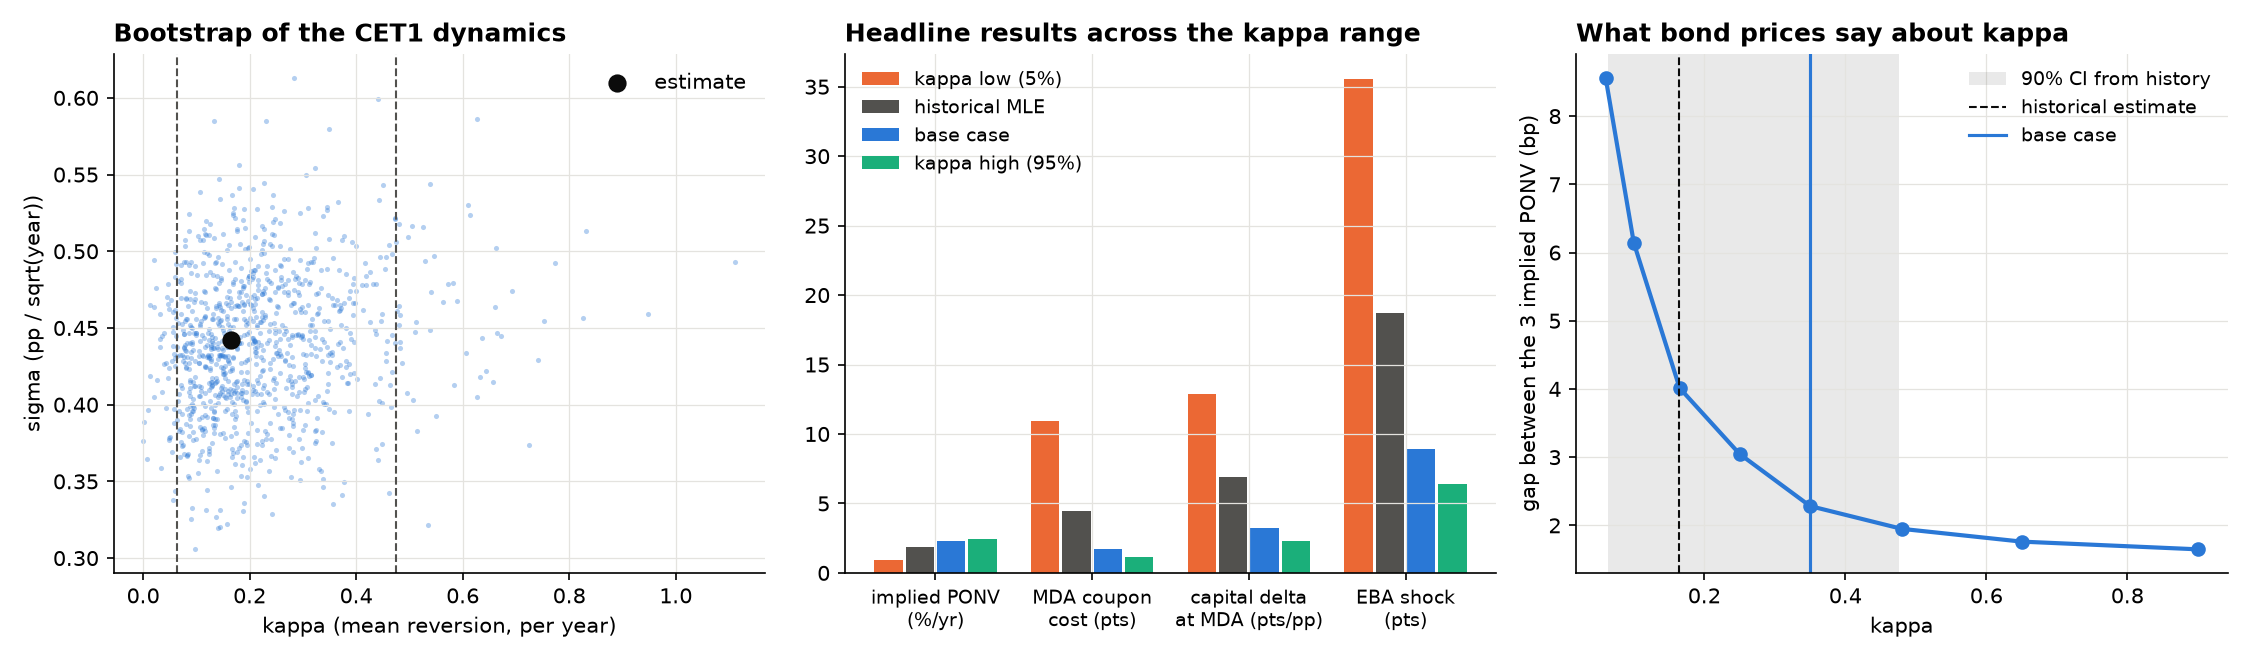
\includegraphics[width=\textwidth]{parameter_uncertainty.png}
\caption{Left: bootstrap of $(\kappa,\sigma)$. Centre: headline results across the
$\kappa$ range. Right: cross-bond dispersion of the implied hazard against $\kappa$.}
\end{figure}

\textbf{What prices add.} History and prices pull in opposite directions. The
three bonds are mutually consistent only for fast capital rebuilding: $D$ falls
from 8.6bp at $\kappa=0.06$ to 1.9bp at $0.48$ and then flattens. The history,
however, rejects values much above 0.35. The base case $\kappa=0.35$
(half-life two years) lies inside the historical interval and close to the
market plateau. It is also consistent with BNP's active capital management (a
13\% target, managed RWA and distributions). The ordering of the bonds, the
extension ranking and the steepening of the capital delta near the MDA threshold
hold across the whole range. The level of the capital stress and the
premium--MDA split do not, and are reported with this range.

\textbf{Where the uncertainty sits.} Each curve in Figure~\ref{fig:cliffunc} is
re-calibrated to today's price of the 6.875\%, so all four scenarios agree at
today's $13\%$ CET1 (94.4). They separate only as capital falls: at the MDA
threshold the price ranges from 80 ($\kappa=0.06$) to 93 ($\kappa=0.48$), and at
$6\%$ CET1 from 36 to 79. Prices identify the level of risk today, not the shape
of the cliff.
\begin{figure}[H]
\centering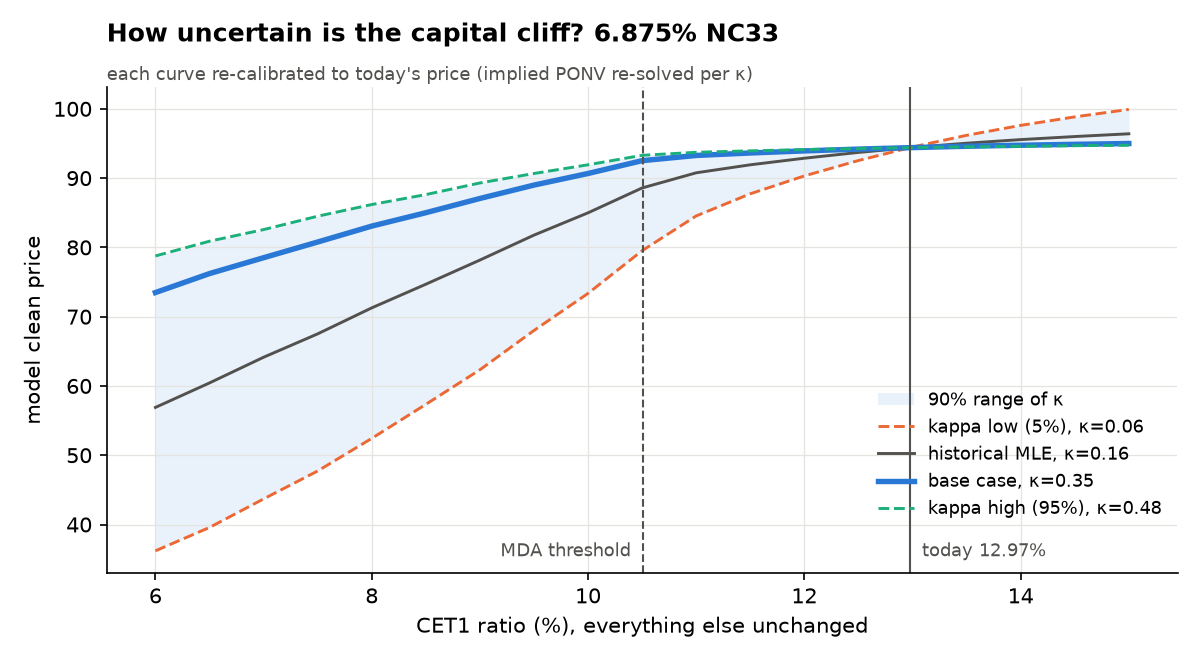
\includegraphics[width=0.8\textwidth]{capital_cliff_uncertainty.png}
\caption{Price of the 6.875\% NC33 against CET1 for four values of $\kappa$, each
re-calibrated to today's price. Shaded: 90\% bootstrap range of $\kappa$.}
\label{fig:cliffunc}
\end{figure}

%======================================================================
\section{Limitations and extensions}
%======================================================================
\begin{enumerate}
  \item \textbf{Measure.} CET1 is not traded. Its dynamics are estimated under
  the physical measure, and all remaining risk premia are absorbed by $\lambda$,
  which is therefore a risk-neutral hazard, not a default probability.
  \item \textbf{Capital mean reversion.} $\kappa$ is weakly identified by 50
  quarters of history and drives the capital stress results
  (\S\ref{sec:uncert}); the base case combines history and prices.
  \item \textbf{Rates.} Today's FRED curve is used for all future resets; a
  short-rate model (Hull--White) would add rate-driven extension.
  \item \textbf{Spread volatility.} $\eta$ is not pinned down by the cross-section.
  \item \textbf{Capital premium.} $\beta$ controls the size of the capital cliff
  and is assumed. A cross-bank regression of AT1 spreads on MDA distance would
  calibrate it.
  \item \textbf{Data.} Prices are evaluated rather than traded, and cover
  15 months of tight spreads.
  \item \textbf{Conversion.} A single stressed share price replaces a joint
  equity--capital process, and PONV recovery is set to zero.
\end{enumerate}

\appendix
\section{Parameters}
\begin{center}
\small
\begin{tabular}{llll}
\toprule
Symbol & Meaning & Value & Source \\
\midrule
$\kappa,\sigma$ & CET1 mean reversion, volatility & 0.35, 0.47pp & MLE 0.165/0.44; base (\S\ref{sec:uncert}) \\
$\theta$ & CET1 target & 13\% & BNP strategic plan \\
$\lambda_J, m_J, \sigma_J$ & stress jumps & 0.12, 2.2pp, 0.5 & EBA 2025 check \\
$b, w$ & MDA floor, combined buffer & 5.64\%, 4.87\% & requirement stack \\
$\ctrig$ & trigger & 5.125\% & term sheets \\
$a, \bar s, \eta, \rho$ & spread OU & 0.5, 275bp, 100bp, $-0.3$ & sample, assumption \\
$\beta$ & capital premium & 1\% per pp & assumption \\
$\xi$ & share at trigger / today & 0.2 & assumption \\
$\lambda$ & PONV hazard today & $\approx2.3\%$ & implied \\
\bottomrule
\end{tabular}
\end{center}

\section{Code map}
\begin{center}
\small
\begin{tabular}{ll}
\toprule
File & Content \\
\midrule
\texttt{processes.py} & CET1 jump-diffusion \eqref{eq:cet1}, trigger times \\
\texttt{instrument.py} & MDA schedule \eqref{eq:mda}, stylised term sheet \\
\texttt{pricer.py}, \texttt{risk.py} & original engine, Greeks, loss distribution \\
\texttt{market.py} & dated bonds, \eqref{eq:spread}--\eqref{eq:hazard}, pricing \eqref{eq:cmc}, implied $\lambda$ \\
\texttt{calibrate\_bnp.py} & calibration (\S\ref{sec:calib}) \\
\texttt{spread\_and\_stress.py} & decomposition, call analysis, stress \\
\texttt{parameter\_uncertainty.py} & bootstrap, $\kappa$ sensitivity (\S\ref{sec:uncert}) \\
\bottomrule
\end{tabular}
\end{center}

\end{document}
